\section{Finite-length Structured SPIN}
\label{sec:finite-certificates}

For practical lengths, a compact fixed outer can give both a fast circuit
and a strong finite guarantee. We first examine how the message length,
outer length, and inner parameters affect the finite bound. We then give
certified rate-$1/2$ and rate-$1/4$ BCH constructions with IMT.

\subsection{How the parameters affect the margin}
\label{sec:finite-parameter-slices}

Consider a rate-$1/2$ outer constituent of length $B$, repeated over
$L=2K/B$ rows to encode $K$ message bits. The output length is $N=2K$.
The IMT inner processes $t$ bits per step, carries an $s$-bit state,
and applies one transvection per update. We ask how to choose $t$ and $s$
as $K$ changes, rather than prescribing one inner for every length.
Throughout the plots, the bad-word cutoff is $H=\lfloor N/10\rfloor$.
For an upper bound $U$ on the expected number of nonzero messages with
output weight at most $H$, call $-\log_2U$ its \emph{margin} in bits.
A full bound includes every number $q$ of active outer rows. Write $U_1$
for an upper bound on the contribution from messages with exactly one
active row, and call $-\log_2 U_1$ the \emph{Q1 margin}.
We use Q1 to explore parameter sensitivity, then compare it with full
certificates at five selected operating points in
Section~\ref{sec:finite-engineering-curve}. Q1 alone does not control
distance failure: messages with two or more active rows remain to be bounded.

Figure~\ref{fig:finite-k-b} centers this comparison on the BCH-derived
$[256,128]$ constituent and implemented $(t,s)=(128,19)$ maps specified in
Section~\ref{sec:finite-selected-construction}. Two smaller exact-spectrum
constituents provide outer-size comparisons: a shortened BCH-derived
$[64,32,12]$ code and an extended BCH $[128,64,22]$ code, called BCH-64
and BCH-128. Their fixed-step curves use $(t,s)=(64,20)$.
For each fixed curve, an ideal mixing reference replaces every transvection
by an independently sampled uniform invertible linear map. Every fixed
nonzero state then has a uniform nonzero image; zero stays zero.
This \emph{full refresh} keeps the outer, routing, expansion, and feedback
fixed. Its Q1 bound is a reference, not an absolute outer-only ceiling.

% Generated by paper/build_imt_parameter_figures.py; do not hand edit.
% Q1 grid SHA-256: 1a48a6f4d5a4c6c1449f35cd7e5584b7a14d4a08f8effc2c4508497e8ef20058
\begin{figure}[!hbp]
\centering
\begin{minipage}[t]{\linewidth}
\centering
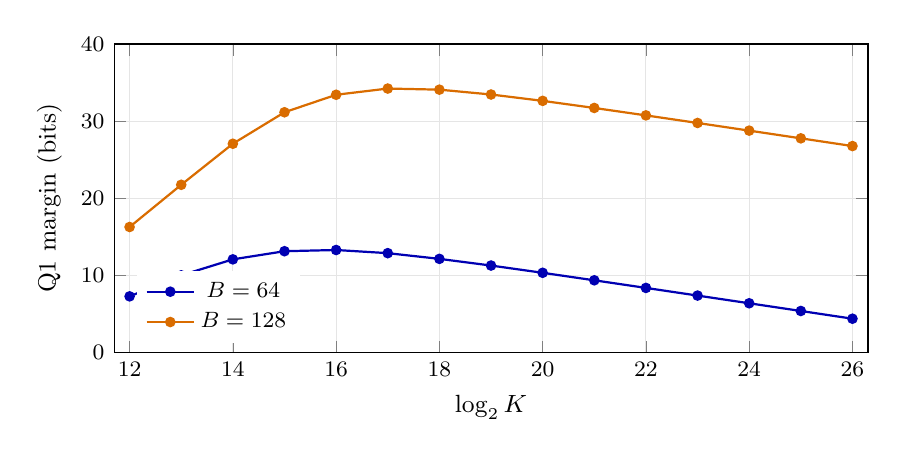
\begin{tikzpicture}
\begin{axis}[tick label style={font=\footnotesize},label style={font=\small},title style={font=\small},grid=major,grid style={black!10},legend style={font=\footnotesize,draw=none},width=.92\linewidth,height=5.5cm,xlabel={$\log_2 K$},ylabel={Q1 margin (bits)},xmin=11.7,xmax=26.3,ymin=0,ymax=40,xtick={12,14,16,18,20,22,24,26},legend pos=south west,]
\addplot[blue!70!black,thick,mark=*,mark size=1.5pt] coordinates {(12,7.2854857489) (13,10.0090201085) (14,12.0832614441) (15,13.1390922468) (16,13.2963998191) (17,12.8871610268) (18,12.1466382431) (19,11.2810369722) (20,10.3403771086) (21,9.3679471183) (22,8.3815223483) (23,7.3876553599) (24,6.3899560564) (25,5.3901051543) (26,4.3889026631)};
\addlegendentry{$B=64$}
\addplot[orange!85!black,thick,mark=*,mark size=1.5pt] coordinates {(12,16.2784460297) (13,21.7503698500) (14,27.0735386208) (15,31.1534629535) (16,33.4221485975) (17,34.2276637311) (18,34.0849090219) (19,33.4552570471) (20,32.6317852093) (21,31.7117191602) (22,30.7488362012) (23,29.7657818858) (24,28.7725947112) (25,27.7739122608) (26,26.7719414261)};
\addlegendentry{$B=128$}
\end{axis}
\end{tikzpicture}
\end{minipage}
\caption{IMT one-active-row bounds versus message length, with $(t,s)=(64,20)$.
The two outers share the same maps. These binary64 Q1 evaluations do not
include higher occupancies. Markers are evaluated configurations;
connecting segments are visual guides in all three parameter-slice figures.}
\label{fig:finite-k-b}
\end{figure}


\paragraph{Why the length curve turns down.}
The Q1 sum contains $L$ possible active rows. Once the bounds on conditional
low-weight probabilities stabilize, doubling $K$, and hence $L$, costs
approximately one margin bit. The larger-length portions of
Figure~\ref{fig:finite-k-b} follow this trend. At short lengths, however,
the conditional probabilities also change: a region contains only
$h:=L/t=2K/(Bt)$ inner steps. At $K=2^{16}$, the BCH-256 fixed-step
configuration has $h=4$, compared with $h=64$ at $K=2^{20}$.
Increasing $B$ at fixed $K,t$ also reduces $h$: a stronger outer can
require a different inner calibration, not just a vertical shift of the curve.

One mechanism is a short excursion away from state zero. The first input
bit injects a nonzero state; a later bit can cancel it before much weight
has been emitted. A transvection retains any fixed nonzero incoming state
with mixture weight $1/2$. After $d$ empty updates, the retained component
therefore has weight $2^{-d}$; it is not a fresh uniform state.
Consider two adjacent regions, each containing one input bit, with zero
state before the first. Let their input positions be independent and
uniform, and suppose the feedback columns are distinct and nonzero.
The probability that the state returns to zero just after the second input is
\[
 p_{\mathrm{cancel}}
 =\frac{\rho_h}{t}+\frac{1-\rho_h}{2^s-1},
 \qquad \rho_h:=\frac{2(1-2^{-h})^2}{h^2}.
\]
The first term comes from repeating the same feedback column while the
state is retained. Increasing $s$ reduces the second term, not the first.
For large $h$, the first term is approximately $2t/L^2$.
These retained cancellations favor inputs near the shared region boundary:
their mean separation approaches three epochs even as $h$ grows.
They can therefore produce short output pulses, rather than benefiting
from the typical number of mixing updates.
This is a local cancellation probability, not a whole-code distance bound;
the emitted weights and all activation patterns still matter.

Additional mixing within each update also suppresses retention. Applying
$r$ independent transvections before adding feedback reduces the retained
component's weight from $1/2$ to $2^{-r}$, without changing the step or maps.
In a separate controlled BCH-256 study with $(t,s)=(128,19)$, increasing
$r$ from one to two raises the Q1 margin from $44.26$ to $51.21$ bits at
$K=2^{16}$. At $K=2^{20}$, the same change gives only $50.08$ to $50.35$
bits: the benefit diminishes once one transvection per update provides
sufficient mixing for these Q1 bounds. The artifact's
\artifactlink{https://github.com/ladnir/permute_conv/blob/main/workstreams/inner_design/finite_migration/MIXING_ROUNDS.md}{mixing-study guide}
records the fixed maps and outward-bound replay. These gains concern Q1,
not full certificates. We keep one transvection per update in the plotted
constructions and instead vary the step, which also changes feedback
grouping and the expansion maps.

\paragraph{Reducing the step at short lengths.}
The adaptive curves keep one transvection per update and select among
smaller steps. At each tested $K$, we take the largest $t$ within $0.1$
bits of the best tested Q1 margin. This tolerance avoids selecting a
smaller step for a negligible bound improvement; it is not a runtime optimum.
For BCH-256, the selected pairs are $(16,10)$ at $K=2^{14}$, $(32,15)$
at $K=2^{16},2^{18}$, and the implemented $(128,19)$ pair at the three
larger tested lengths. At $K=2^{16}$, the smaller step improves Q1 from
$44.36$ to $49.04$ bits. For BCH-128 at $K=2^{12}$, it improves Q1 from
$19.18$ to $24.27$ bits. The short-length loss shrinks but does not disappear.

Shrinking $t$ has a competing cost in this map family. With $t=2^m$,
the nonconstant degree-at-most-two generators span only $m+\binom m2$
dimensions. Our $t=32,16,8$ candidates consequently use $s=15,10,6$.
Smaller state spaces increase fresh-state cancellation probabilities, and
different expansion maps change the emitted-weight distribution.
Indeed, $t=8$ wins at none of the tested lengths. There is no evidence here
for a universal rule based only on $K/t$.

The artifact's
\artifactlink{https://github.com/ladnir/permute_conv/blob/main/workstreams/inner_design/finite_migration/ADAPTIVE_LENGTH.md}{length-study guide}
specifies all maps, derives the local cancellation formula, and records
the $110$-cell independent log-domain replay. Figure~\ref{fig:finite-k-b}
tracks the expansion-weight shell at activation, sharpening the earlier
diagnostic calculation. At the shortest BCH-128 point this alone improves
the bound by $2.90$ bits; that gain is separate from changing $t$.
The selected BCH-256 certificates below do not certify the different BCH-64/128 diagnostic configurations
or the smaller-step BCH-256 alternatives.

\paragraph{State size and step size.}
Figures~\ref{fig:finite-s-t} and \ref{fig:finite-k-s} retain the broader
BCH-64/128 state study. At each $t$, fixed ordered map chains give nested
state maps; the same maps serve both outer lengths and all $K$.
These slices use the earlier activation envelope. The
\artifactlink{https://github.com/ladnir/permute_conv/blob/main/workstreams/inner_design/finite_migration/PARAMETER_SLICES.md}{state-study guide}
records their $130$ geometries and replay.
Figure~\ref{fig:finite-s-t} fixes $K=2^{20}$. At $t=64$, additional state
first buys substantial margin and then gives diminishing returns.
For BCH-128, increasing $s$ from $10$ to $16$ raises the Q1 margin
from $26.99$ to $32.34$ bits; increasing it to $20$ adds only $0.29$ bits.
Increasing $t$ reduces the number of inner steps, while the Q1 curves
nearly coincide at shared states in this study. At $s=20$, the BCH-128 Q1 margins for
$t\in\{64,128,256\}$ are $32.63$, $32.49$, and $32.46$ bits.
Their closeness does not establish comparable full margins: larger steps
also change the multi-row activation and cancellation bounds.

% Generated by paper/build_imt_parameter_figures.py; do not hand edit.
% Q1 grid SHA-256: 1a48a6f4d5a4c6c1449f35cd7e5584b7a14d4a08f8effc2c4508497e8ef20058
\begin{figure}[tb]
\centering
\begin{minipage}[t]{.485\linewidth}
\centering
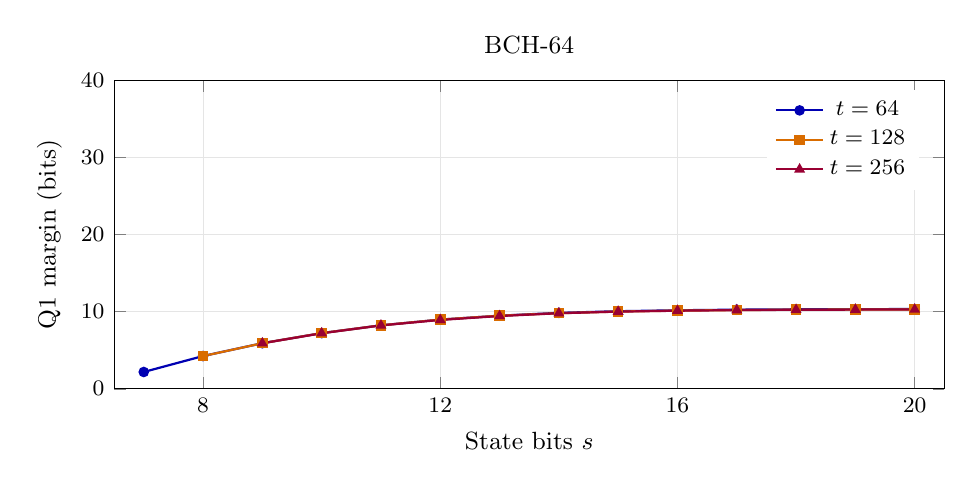
\begin{tikzpicture}
\begin{axis}[tick label style={font=\footnotesize},label style={font=\small},title style={font=\small},grid=major,grid style={black!10},legend style={font=\footnotesize,draw=none},width=\linewidth,height=5.5cm,title={BCH-64},xlabel={State bits $s$},ylabel={Q1 margin (bits)},xmin=6.5,xmax=20.5,ymin=0,ymax=40,xtick={8,12,16,20},legend pos=north east,]
\addplot[blue!70!black,thick,mark=*,mark size=1.5pt] coordinates {(7,2.1827116585) (8,4.2514093897) (9,5.9147821095) (10,7.2247246256) (11,8.2306365668) (12,8.9772543375) (13,9.4838898435) (14,9.8505560891) (15,10.0610100645) (16,10.1847253778) (17,10.2642828362) (18,10.3073487861) (19,10.3292263422) (20,10.3403771086)};
\addlegendentry{$t=64$}
\addplot[orange!85!black,thick,mark=square*,mark size=1.5pt] coordinates {(8,4.2430472521) (9,5.9129395061) (10,7.2224925389) (11,8.2281561682) (12,8.9741001763) (13,9.4805569735) (14,9.8077200834) (15,10.0175657415) (16,10.1370857462) (17,10.2158805444) (18,10.2589462533) (19,10.2808187416) (20,10.2919600489)};
\addlegendentry{$t=128$}
\addplot[purple!80!black,thick,mark=triangle*,mark size=1.5pt] coordinates {(9,5.9089535105) (10,7.2018221055) (11,8.2229102705) (12,8.9322403044) (13,9.4387211691) (14,9.7997939364) (15,10.0090784426) (16,10.1270377235) (17,10.2050661704) (18,10.2479773575) (19,10.2698512751) (20,10.2808321532)};
\addlegendentry{$t=256$}
\end{axis}
\end{tikzpicture}
\end{minipage}
\hfill
\begin{minipage}[t]{.485\linewidth}
\centering
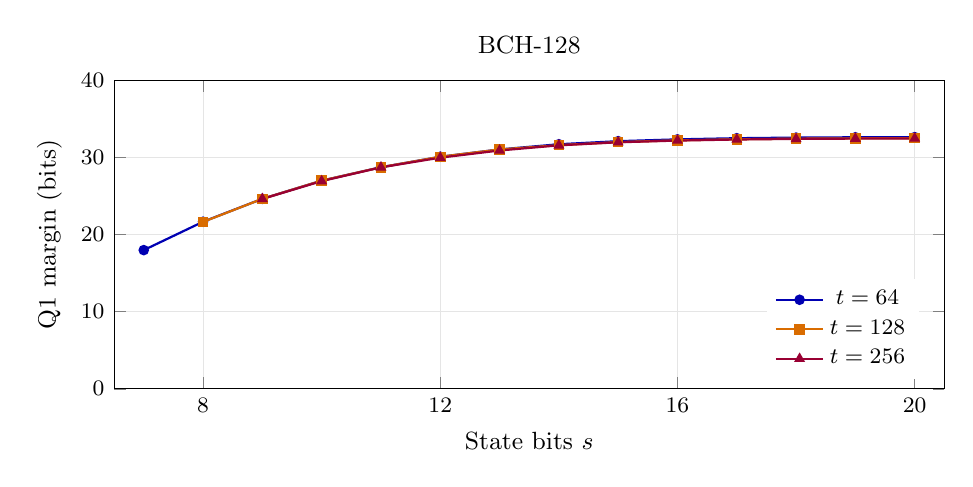
\begin{tikzpicture}
\begin{axis}[tick label style={font=\footnotesize},label style={font=\small},title style={font=\small},grid=major,grid style={black!10},legend style={font=\footnotesize,draw=none},width=\linewidth,height=5.5cm,title={BCH-128},xlabel={State bits $s$},ylabel={Q1 margin (bits)},xmin=6.5,xmax=20.5,ymin=0,ymax=40,xtick={8,12,16,20},legend pos=south east,]
\addplot[blue!70!black,thick,mark=*,mark size=1.5pt] coordinates {(7,17.9834453302) (8,21.6621321145) (9,24.6347504734) (10,26.9894832727) (11,28.7304904965) (12,30.0911153162) (13,31.0377180335) (14,31.7087951291) (15,32.1068469089) (16,32.3411624023) (17,32.4919665503) (18,32.5706569452) (19,32.6109835173) (20,32.6317852093)};
\addlegendentry{$t=64$}
\addplot[orange!85!black,thick,mark=square*,mark size=1.5pt] coordinates {(8,21.6399383579) (9,24.6317302099) (10,26.9854051669) (11,28.7251108759) (12,30.0842904573) (13,31.0283485223) (14,31.5876633568) (15,31.9847921817) (16,32.2093340249) (17,32.3546170480) (18,32.4330203557) (19,32.4731496421) (20,32.4935511435)};
\addlegendentry{$t=128$}
\addplot[purple!80!black,thick,mark=triangle*,mark size=1.5pt] coordinates {(9,24.6251404652) (10,26.9311396417) (11,28.7137024495) (12,29.9699710581) (13,30.9001510687) (14,31.5677999653) (15,31.9634354456) (16,32.1865537842) (17,32.3248385177) (18,32.4027324343) (19,32.4425635106) (20,32.4626971764)};
\addlegendentry{$t=256$}
\end{axis}
\end{tikzpicture}
\end{minipage}
\caption{IMT state and step size at $K=2^{20}$. Each $t$ uses its own nested
map chain. More state gives diminishing Q1 gains; the step-size curves
nearly coincide at shared states.}
\label{fig:finite-s-t}
\end{figure}


\paragraph{State size at larger message lengths.}
Figure~\ref{fig:finite-k-s} compares the state curve at
$K\in\{2^{16},2^{20},2^{24}\}$, holding $t=64$ fixed.
The nearly saturated part shifts downward as $K$ grows, but the loss need
not be a uniform vertical shift. For BCH-128 at $K=2^{24}$, raising $s$
from $10$ to $16$ improves Q1 from $23.04$ to $28.50$ bits; raising it to
$20$ adds only $0.27$ bits.

% Generated by paper/build_imt_parameter_figures.py; do not hand edit.
% Q1 grid SHA-256: 1a48a6f4d5a4c6c1449f35cd7e5584b7a14d4a08f8effc2c4508497e8ef20058
\begin{figure}[tb]
\centering
\begin{minipage}[t]{.485\linewidth}
\centering
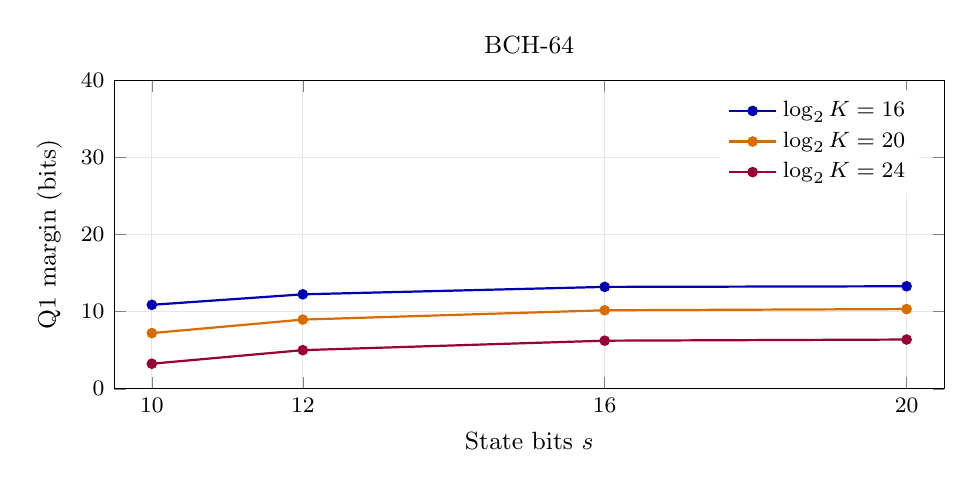
\begin{tikzpicture}
\begin{axis}[tick label style={font=\footnotesize},label style={font=\small},title style={font=\small},grid=major,grid style={black!10},legend style={font=\footnotesize,draw=none},width=\linewidth,height=5.5cm,title={BCH-64},xlabel={State bits $s$},ylabel={Q1 margin (bits)},xmin=9.5,xmax=20.5,ymin=0,ymax=40,xtick={10,12,16,20},legend pos=north east,]
\addplot[blue!70!black,thick,mark=*,mark size=1.5pt] coordinates {(10,10.8900834302) (12,12.2521826982) (16,13.2140320000) (20,13.2963998191)};
\addlegendentry{$\log_2 K=16$}
\addplot[orange!85!black,thick,mark=*,mark size=1.5pt] coordinates {(10,7.2247246256) (12,8.9772543375) (16,10.1847253778) (20,10.3403771086)};
\addlegendentry{$\log_2 K=20$}
\addplot[purple!80!black,thick,mark=*,mark size=1.5pt] coordinates {(10,3.2555009968) (12,5.0147499021) (16,6.2417426575) (20,6.3899560564)};
\addlegendentry{$\log_2 K=24$}
\end{axis}
\end{tikzpicture}
\end{minipage}
\hfill
\begin{minipage}[t]{.485\linewidth}
\centering
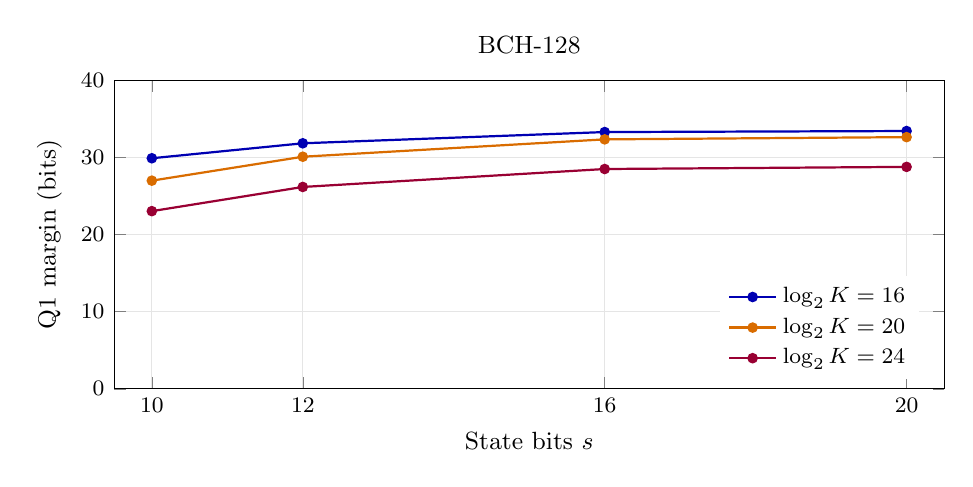
\begin{tikzpicture}
\begin{axis}[tick label style={font=\footnotesize},label style={font=\small},title style={font=\small},grid=major,grid style={black!10},legend style={font=\footnotesize,draw=none},width=\linewidth,height=5.5cm,title={BCH-128},xlabel={State bits $s$},ylabel={Q1 margin (bits)},xmin=9.5,xmax=20.5,ymin=0,ymax=40,xtick={10,12,16,20},legend pos=south east,]
\addplot[blue!70!black,thick,mark=*,mark size=1.5pt] coordinates {(10,29.8922450081) (12,31.8325429428) (16,33.2903309329) (20,33.4221485975)};
\addlegendentry{$\log_2 K=16$}
\addplot[orange!85!black,thick,mark=*,mark size=1.5pt] coordinates {(10,26.9894832727) (12,30.0911153162) (16,32.3411624023) (20,32.6317852093)};
\addlegendentry{$\log_2 K=20$}
\addplot[purple!80!black,thick,mark=*,mark size=1.5pt] coordinates {(10,23.0356798756) (12,26.1715082460) (16,28.4983268727) (20,28.7725947112)};
\addlegendentry{$\log_2 K=24$}
\end{axis}
\end{tikzpicture}
\end{minipage}
\caption{IMT state slices at three message lengths, with $t=64$ fixed.
Only the four marked states are compared at every length. Increasing
message length lowers the Q1 plateau; increasing state gives diminishing gains.}
\label{fig:finite-k-s}
\end{figure}


Together, the slices suggest calibrating $t$ at the intended $K$, then
checking which compatible state maps approach the available Q1 margin.
The choice $s=19$ below is a demonstrated operating point, not a proved
minimum or optimum. The final tests are the full bound over all occupancies
and the cost of the resulting encoder; neither follows from Q1 alone.
\FloatBarrier

\subsection{The selected construction}
\label{sec:finite-selected-construction}

We now use a binary BCH-derived constituent $\mathcal B$ of length $256$,
dimension $128$, and minimum distance at least $38$.
Its exact weight spectrum is unknown. The proof instead uses deterministic
inequalities for that spectrum, with no exceptional event for the choice
of outer.

Let $P$ and $Q$ be the parity extensions of the primitive binary BCH codes
of length $255$ and designed distances $37$ and $39$, respectively.
Their dimensions are $131$ and $123$. The selected constituent satisfies
$Q\subset\mathcal B\subset P$ and has dimension $128$.
Appendix~\ref{app:finite-bch-definition} specifies its generators and explains
why the spectrum bounds apply to the implemented code.

For $K$ message bits, choose
\[
  L:=K/128,\qquad N:=256L=2K,\qquad (t,s):=(128,19).
\]
Use $\mathcal B$ in every outer row and the structured interleaver of
Section~\ref{sec:structured-spin}. Use the IMT maps
$A:\F_2^{19}\to\F_2^{128}$ and $C:\F_2^{128}\to\F_2^{19}$ in
Table~\ref{tab:imt-maps}, also used by the asymptotic construction.
Setup $\theta$ consists of
independent uniform row permutations, independent uniform region permutations,
and independent transvections $M_i=I+u_iv_i^\top$: sample $u_i$ uniformly
from the nonzero state vectors and $v_i$ uniformly from $u_i^\perp$,
including zero.
One setup is shared by all messages.

The inner processes the routed $128$-bit groups $X_i$ in order:
\[
  Q_0=0,\qquad Y_i=X_i+A(Q_i),\qquad
  Q_{i+1}=M_iQ_i+C(X_i).
\]
Output precedes the state update. The state persists across region boundaries,
and the final state is discarded without a flush. There is no parity fanout.
Thus the inner and routing distribution are shared with the asymptotic
construction; the finite guarantee uses a fixed outer and a separate
finite first-moment calculation.

\subsection{Finite distance guarantee}

\begin{samepage}
\begin{theorem}[Certified BCH-256 Structured SPIN]
\label{thm:finite-bch-spin}
\leavevmode\par
For each $K\in\{2^{16},2^{18},2^{20},2^{22},2^{24}\}$, let $E_\theta$ be
the selected encoder above and put $H:=\lfloor N/10\rfloor$.
Every realization is a binary linear code of rate $1/2$, and
\begin{equation}
  \Prob_\theta\!\left[
    \exists x\ne0:\ \wt(E_\theta(x))\le H
  \right]\le U_K<2^{-40}.
  \label{eq:finite-bch-distance}
\end{equation}
The certified bounds $U_K$ have the margins reported in
Table~\ref{tab:finite-bch-margins}.
\end{theorem}
\end{samepage}

\begin{table}[tb]
\centering
\caption{Complete finite certificates for the selected $(128,19)$ IMT inner.
Margins are rounded for display; the theorem uses exact rational upper bounds.}
\label{tab:finite-bch-margins}
\begin{tabular}{@{}rrrr@{}}
\toprule
$\log_2K$ & outer rows $L$ & cutoff $H$ & $-\log_2U_K$ (bits) \\
\midrule
16 & 512 & 13\,107 & 41.818327 \\
18 & 2\,048 & 52\,428 & 50.189076 \\
20 & 8\,192 & 209\,715 & 50.062088 \\
22 & 32\,768 & 838\,860 & 48.390492 \\
24 & 131\,072 & 3\,355\,443 & 46.457255 \\
\bottomrule
\end{tabular}
\end{table}

Thus, except with probability below $2^{-40}$ over setup, every nonzero
message has output weight greater than $N/10$.
The margin measures a certified upper bound on distance failure, not the
true failure probability or the security level of a complete application.
The theorem covers the five listed lengths, rather than every length between
them. It does not assert an asymptotic distance guarantee for fixed
$\mathcal B$ and fixed inner parameters.

\paragraph{Proof overview.}
Let $Z_H$ count nonzero messages whose output weight is at most $H$.
Partition messages by the number $q$ of nonzero outer rows and by their
row-weight classes. The first-moment framework gives
\begin{equation}
  \Prob_\theta[Z_H>0]\le\E_\theta Z_H
  \le\sum_{\tau\in\mathcal T}
      \widehat A_\tau^{\mathrm{out}}\widehat Q_\tau(H)
  =:U_K.
  \label{eq:finite-certificate}
\end{equation}
Here $\widehat A_\tau^{\mathrm{out}}$ bounds the class multiplicity and
$\widehat Q_\tau(H)$ bounds its conditional failure probability.
No independence between different codewords is required.

The $q=1$ contribution combines a positive inner transfer calculation with
weighted BCH spectrum inequalities. Sparse occupancies use a positive
polynomial recurrence that retains the region-weight constraint. Dense
occupancies use a comparison with independent Bernoulli inputs, together
with input and output tilts. The all-one outer word is counted separately:
its exact multiplicity and deterministic support must not be inflated by an
ordinary weight-band envelope.

For the three largest instances, the sparse recurrence covers $2\le q\le511$,
and interval certificates cover $512\le q\le L$. The two smaller instances
use a lower sparse cutoff and sharper routing-density comparisons, with
separate bounds for assignments containing high-weight rows. All contributions are
included in an exact rational union. Appendix~\ref{app:finite-bch-proof}
gives the mathematical reductions and identifies the bound inputs and
coverage checks.

\subsection{The certified engineering curve}
\label{sec:finite-engineering-curve}

Figure~\ref{fig:finite-bch-curve} holds the outer and selected inner fixed
and compares the Q1 component with the complete certificate at each length.
Between $2^{20}$ and $2^{24}$, the full bound falls from $50.062$ to
$46.457$ bits, roughly $0.90$ bits per doubling. This is a local description
of the certified points, not a bound at an untested length. At $K=2^{16}$,
the Q1 margin is already lower, at $43.593$ bits. Adding the higher-occupancy
bounds costs another $1.775$ bits, giving the full margin of $41.818$ bits;
the dense contribution dominates this additional loss. The short-length
dip therefore occurs in Q1 as well as in the full bound.
At each of the four larger tested lengths, the Q1-to-full loss is below
$0.0002$ bits.
Thus Q1 closely describes the selected certified curve beyond its
short-length transient. This comparison concerns upper bounds, not the
tightness of either bound against the true failure probability.

% Generated by paper/build_imt_parameter_figures.py; do not hand edit.
% Q1 grid SHA-256: 1a48a6f4d5a4c6c1449f35cd7e5584b7a14d4a08f8effc2c4508497e8ef20058
\begin{figure}[tb]
\centering
\begin{minipage}[t]{\linewidth}
\centering
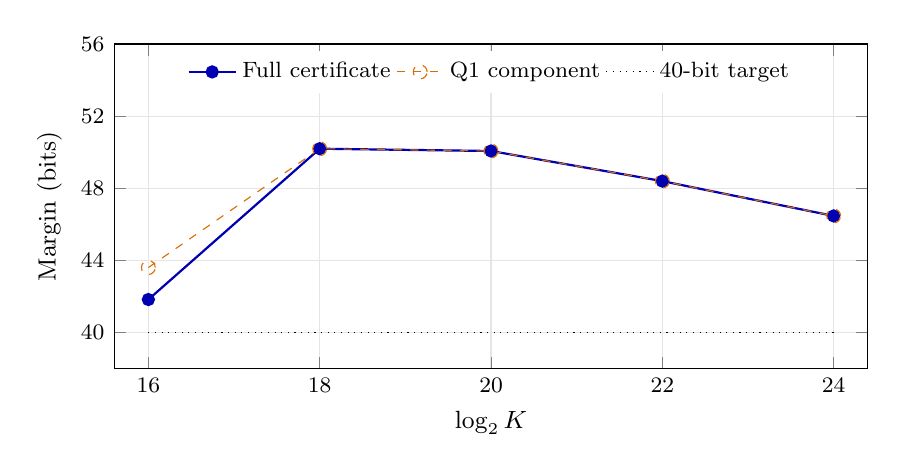
\begin{tikzpicture}
\begin{axis}[tick label style={font=\footnotesize},label style={font=\small},title style={font=\small},grid=major,grid style={black!10},legend style={font=\footnotesize,draw=none},width=.92\linewidth,height=5.7cm,xlabel={$\log_2 K$},ylabel={Margin (bits)},xmin=15.6,xmax=24.4,ymin=38,ymax=56,xtick={16,18,20,22,24},ytick={40,44,48,52,56},legend style={at={(.5,.98)},anchor=north,legend columns=3},]
\addplot[blue!70!black,thick,mark=*,mark size=2pt] coordinates {(16,41.8183267960) (18,50.1890763816) (20,50.0620882264) (22,48.3904916829) (24,46.4572549297)};
\addlegendentry{Full certificate}
\addplot[orange!85!black,dashed,mark=o,mark size=2.5pt] coordinates {(16,43.5928335021) (18,50.1891811139) (20,50.0622720959) (22,48.3904952900) (24,46.4572568186)};
\addlegendentry{Q1 component}
\addplot[black,dotted] coordinates {(16,40.0000000000) (24,40.0000000000)};
\addlegendentry{40-bit target}
\end{axis}
\end{tikzpicture}
\end{minipage}
\caption{Matched Q1 components and complete outward bounds for the selected
BCH-256, IMT $(128,19)$ construction. Both curves use exactly the same
maps and setup distribution. The four larger-length pairs nearly coincide.
Connecting segments do not certify intermediate lengths.}
\label{fig:finite-bch-curve}
\end{figure}


Section~\ref{sec:finite-parameter-slices} investigates smaller steps as
an alternative at short lengths. All certificates here and the measured
implementations retain $(t,s)=(128,19)$ and one transvection per update.

These certified margins are conservative inputs to a parameter selector.
A heuristic estimate of the unknown BCH spectrum addresses a different
question: how much slack remains in those inputs? Backtests on smaller
known-spectrum constituents can support such estimates, but do not bound
their error for BCH-256.

\subsection{A quarter-rate operating point}
\label{sec:finite-quarter}

At rate $1/4$, use the fixed BCH-derived $[128,32,32]$ constituent specified
in Appendix~\ref{app:finite-quarter-definition}. Its spectrum is known
exactly. Set $K=2^{20}$, $L=K/32$, and $N=128L=4K$. Keep the same
routing distribution, expansion $A$, $(t,s)=(128,19)$, and transvection
law. Use the weight-three feedback map in
Table~\ref{tab:finite-quarter-feedback}. Only the outer and feedback map
change; the inner recurrence and end conditions are unchanged.

\begin{theorem}[Certified quarter-rate SPIN]
\label{thm:finite-quarter-spin}
For this encoder, every setup gives a binary linear code of rate $1/4$.
For either row of Table~\ref{tab:finite-quarter-margins},
\[
 \Prob_\theta[\exists x\ne0:\wt(E_\theta(x))\le\lfloor\delta N\rfloor]
 \le U_\delta<2^{-\lambda}.
\]
\end{theorem}

\begin{table}[tb]
\centering
\caption{Two distance thresholds for the same quarter-rate encoder at
$K=2^{20}$. The exact unions, not the rounded margins, establish the targets.}
\label{tab:finite-quarter-margins}
\begin{tabular}{@{}rrrr@{}}
\toprule
$\delta$ & cutoff $\lfloor\delta N\rfloor$ & target $\lambda$ & margin (bits) \\
\midrule
0.165 & 692\,060 & 40 & 41.048168 \\
0.190 & 796\,917 & 30 & 30.033491 \\
\bottomrule
\end{tabular}
\end{table}

The proof uses the same IMT transfer with the separately enumerated feedback
spectrum and cancellation data, followed by a complete sum over
$1\le q\le32768$. These two bounds concern different distance thresholds
for one setup distribution, not two independently selected inner designs.
